\subsection{Encoding via EfficientNetV2L}
Observing Figure \ref{fig:efficientnetv2l_learning_curve}, the learning curves of the
EfficientNetV2L model, there is a change in the patterns seen among the other models.
The curves are comparable in terms of general characteristics, the starting and resulting losses are
comparable and the majority is reduced in the first few epochs.
In detail however the variance of the validation losses do not show a further increase,
it steadily follows the training curve.
Also for this model there is no overfitting or any training issue detected, the training data
seem to represent the whole dataset, this is supported by the validation curve.

\begin{figure}[!ht]
    \centering
    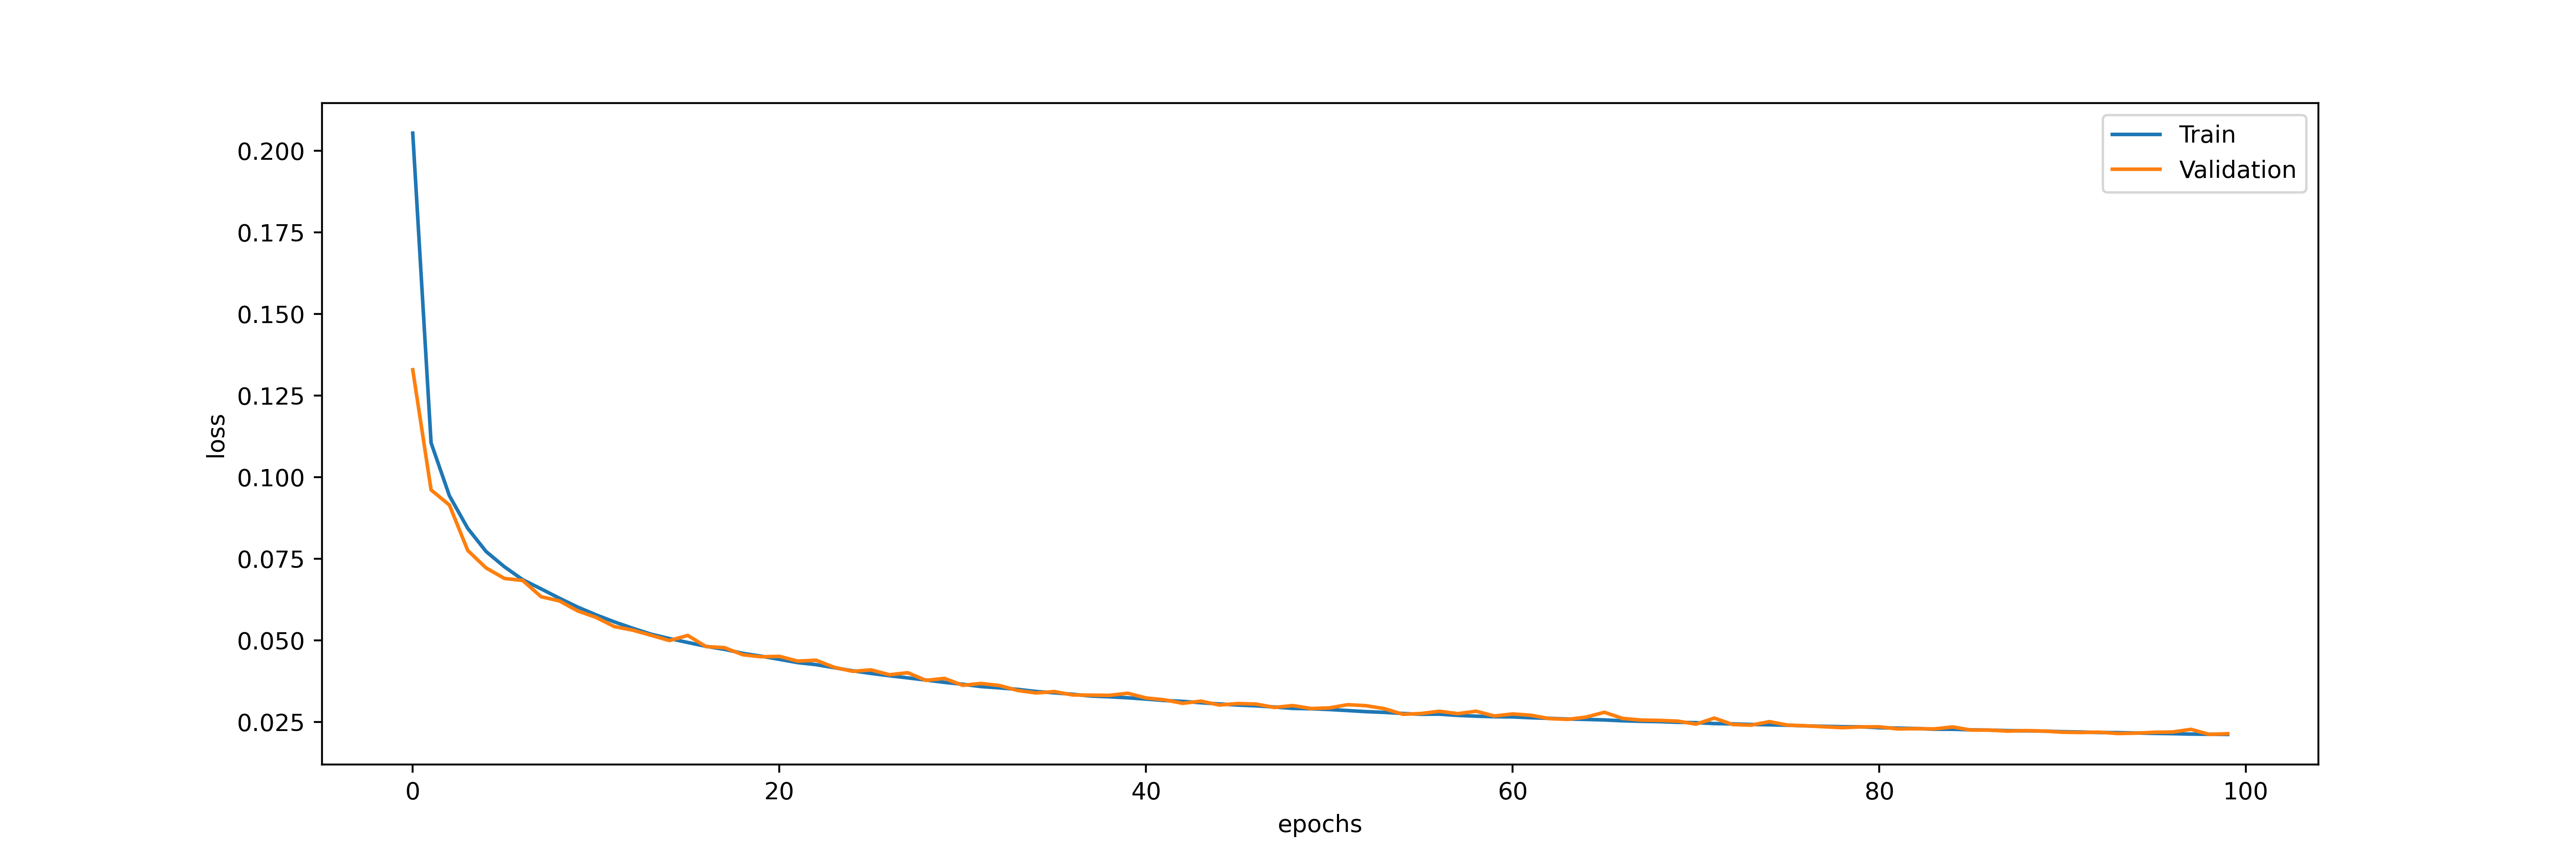
\includegraphics[width=\textwidth,trim={0 0 0 1cm},clip]{./results/efficientnetv2l_vgg19/20230525_194238_results.png}
    \caption{Learning curve of the EfficientNetV2L Encoder}
    \label{fig:efficientnetv2l_learning_curve}
\end{figure}

The predicted images are similar to the ones seen before, the basic features are well grabbed and
the details are focusing around the center or bright part of the images.
The rail itself and ballast stones can be easily recognised, the model (same as for the other models)
captures the edges easily.
The reconstructed images however still not deliver full pictures, loss of information due to
incompleteness is assumed.
The sample images are presented on Figure \ref{fig:efficientnetv2l_examples}

\begin{figure}[!ht]
    \centering
    \begin{subfigure}{\textwidth}
        \centering
        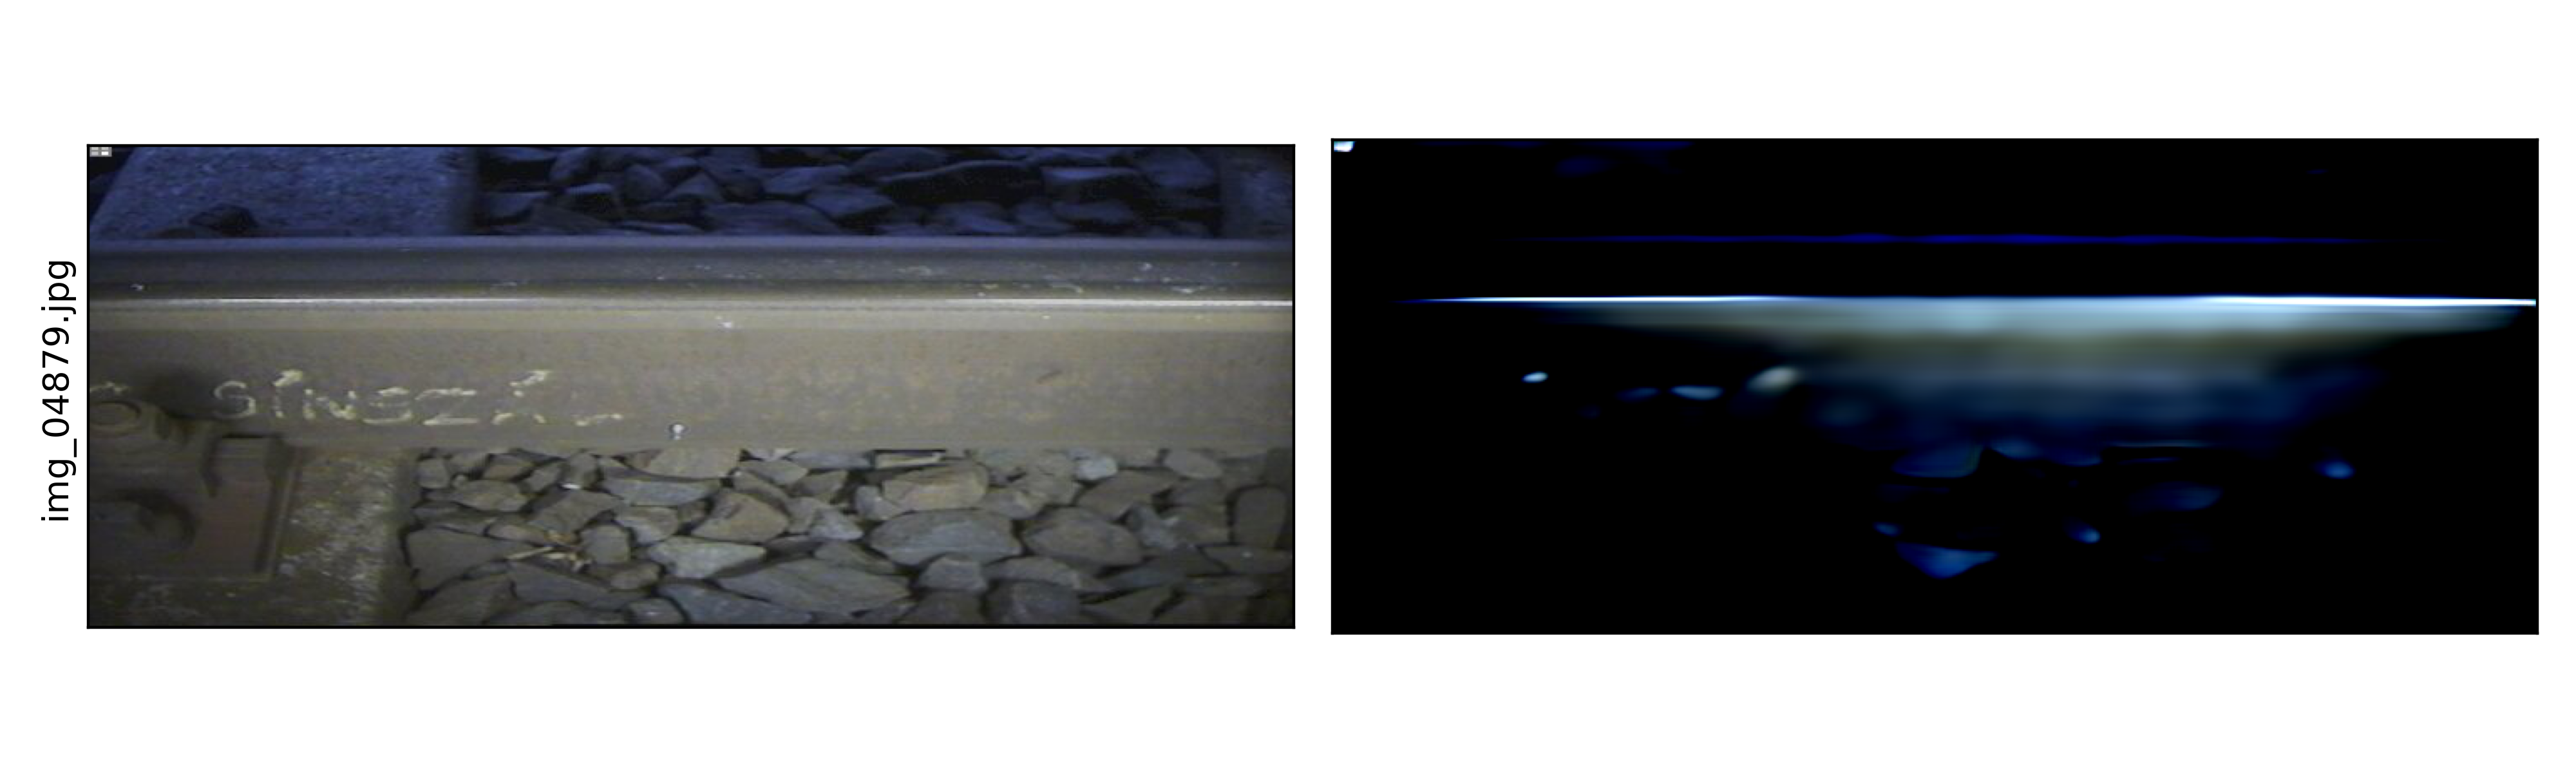
\includegraphics[width=0.9\textwidth,trim={0 1cm 0 1cm},clip]{./results/efficientnetv2l_vgg19/20230525_194238_predict_0.png}
    \end{subfigure}
    \begin{subfigure}{\textwidth}
        \centering
        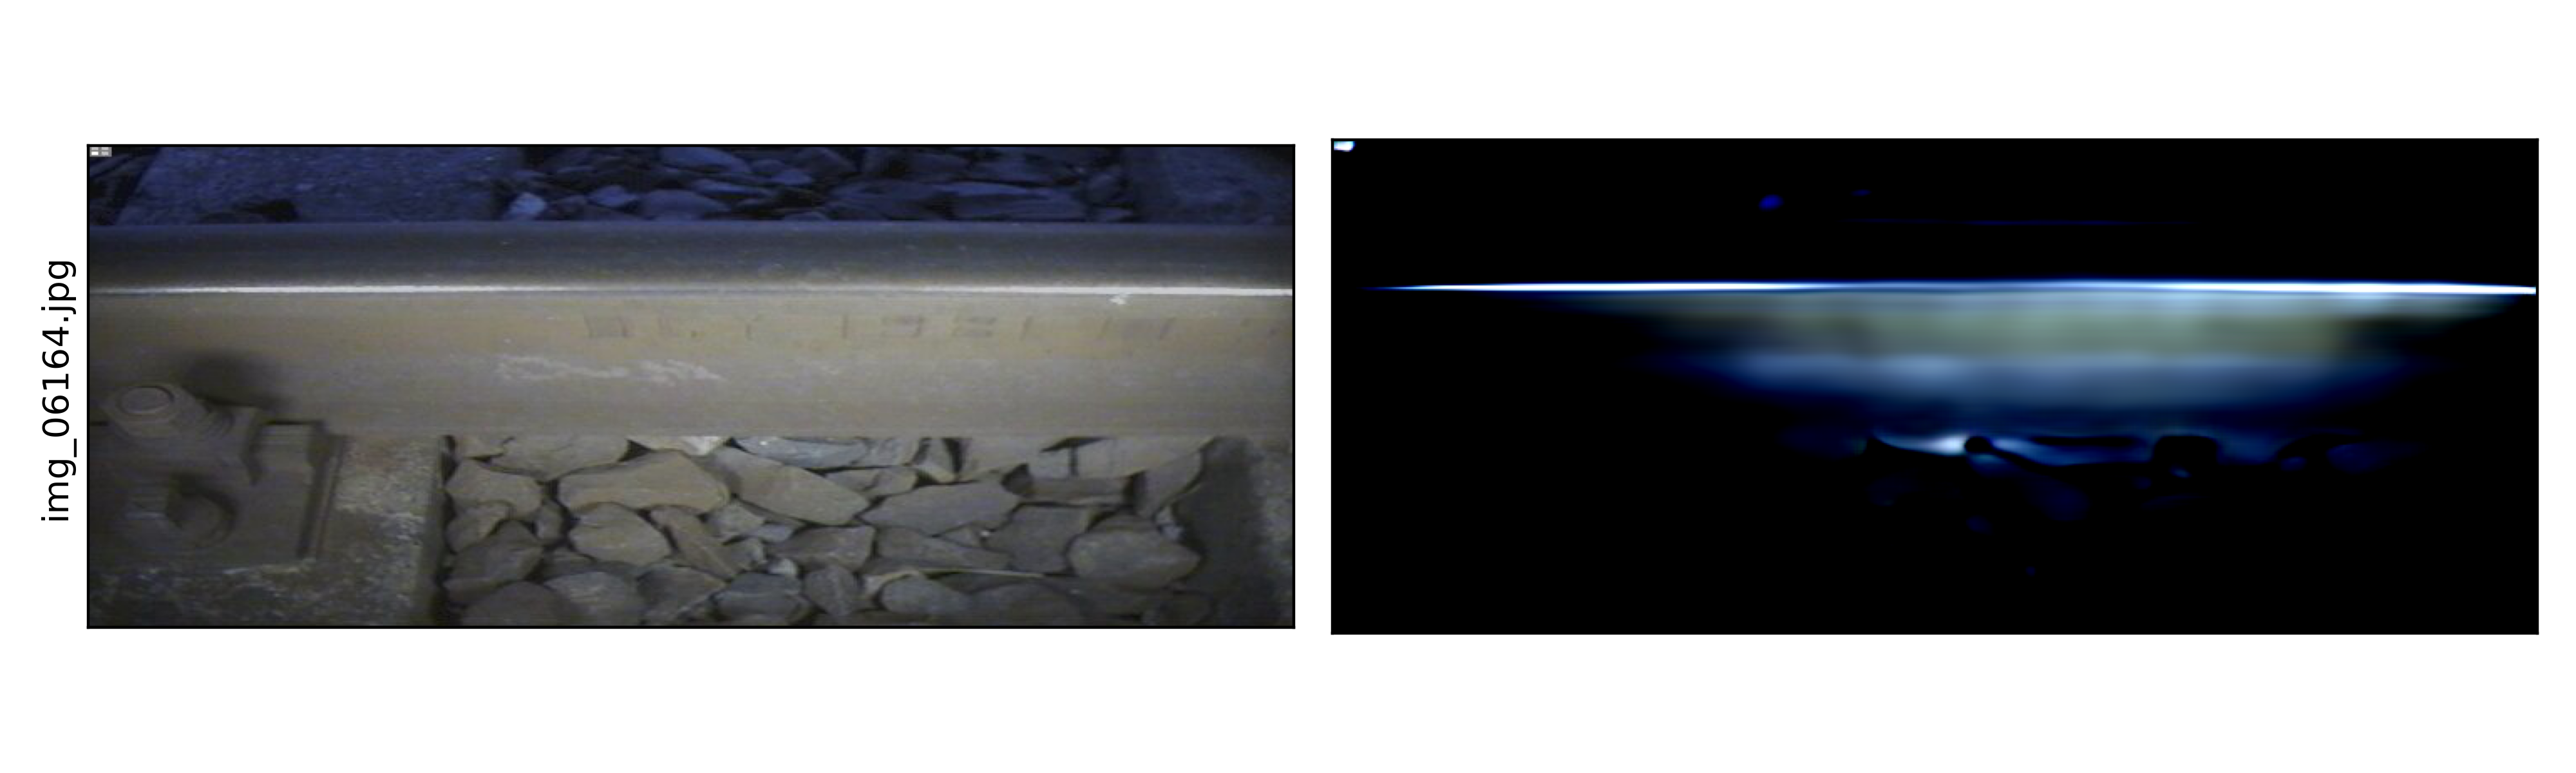
\includegraphics[width=0.9\textwidth,trim={0 1cm 0 1cm},clip]{./results/efficientnetv2l_vgg19/20230525_194238_predict_1.png}
    \end{subfigure}
    \begin{subfigure}{\textwidth}
        \centering
        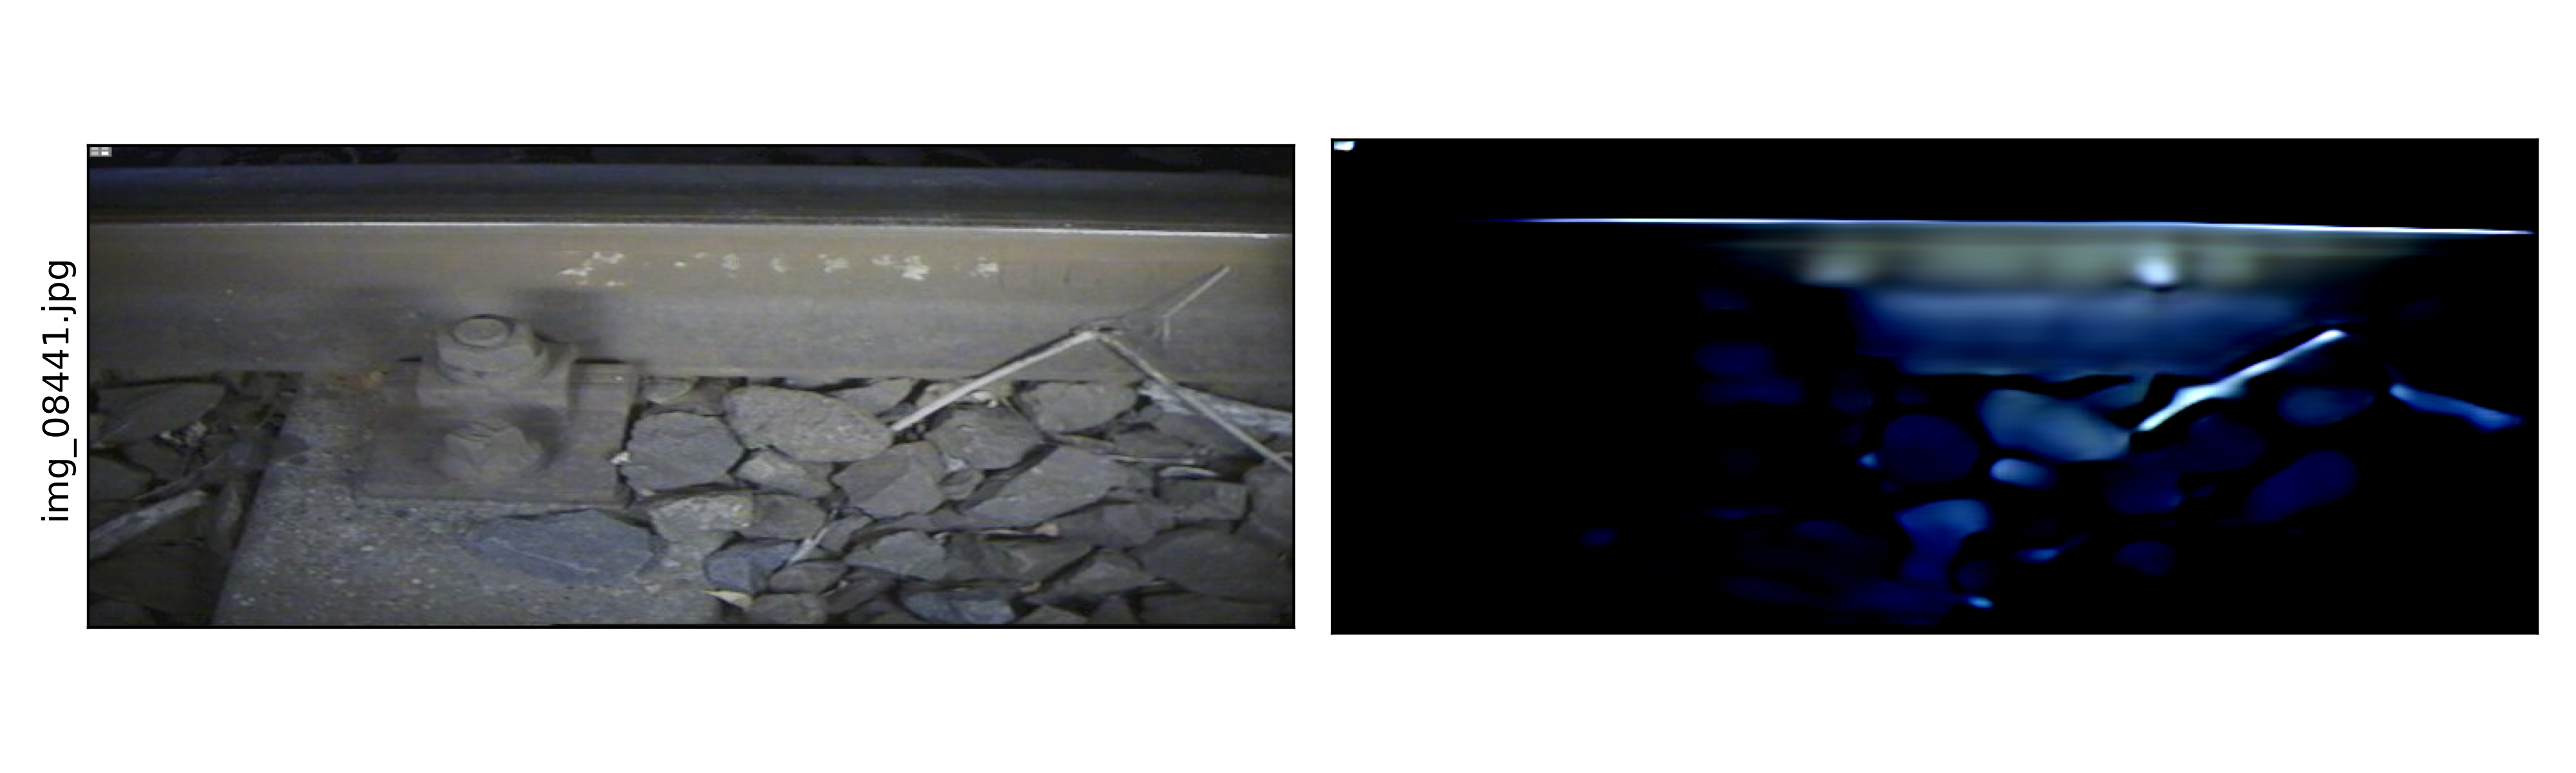
\includegraphics[width=0.9\textwidth,trim={0 1cm 0 1cm},clip]{./results/efficientnetv2l_vgg19/20230525_194238_predict_2.png}
    \end{subfigure}
    \caption{Predicted images in case of EfficientNetV2L Encoder}
    \label{fig:efficientnetv2l_examples}
\end{figure}

Reducing the dimensions to a plane results comparable characteristic behaviour as the other models
as shown on Figure \ref{fig:efficientnetv2l_pca}.
Although there are some differences that need to be noted.
First, the outliers are captured and separated from the \emph{normal} cluster, especially on the
bottom right part of the encoded view, however the separation is not as clear as was for example
in case of the ResNet50 Encoder.
Secondly the outliers that are stucked on the top right part of the encoded view inside the \emph{normal}
cluster are now moved more to the boundary and even the \emph{normal} cluster is opened up better.
After decoding back the images, the resulting feature plane shows that the outliers are placed back
more concentrated to their original place indicating a certain loss of information
and generalization of the model.

\begin{figure}[!ht]
    \centering
    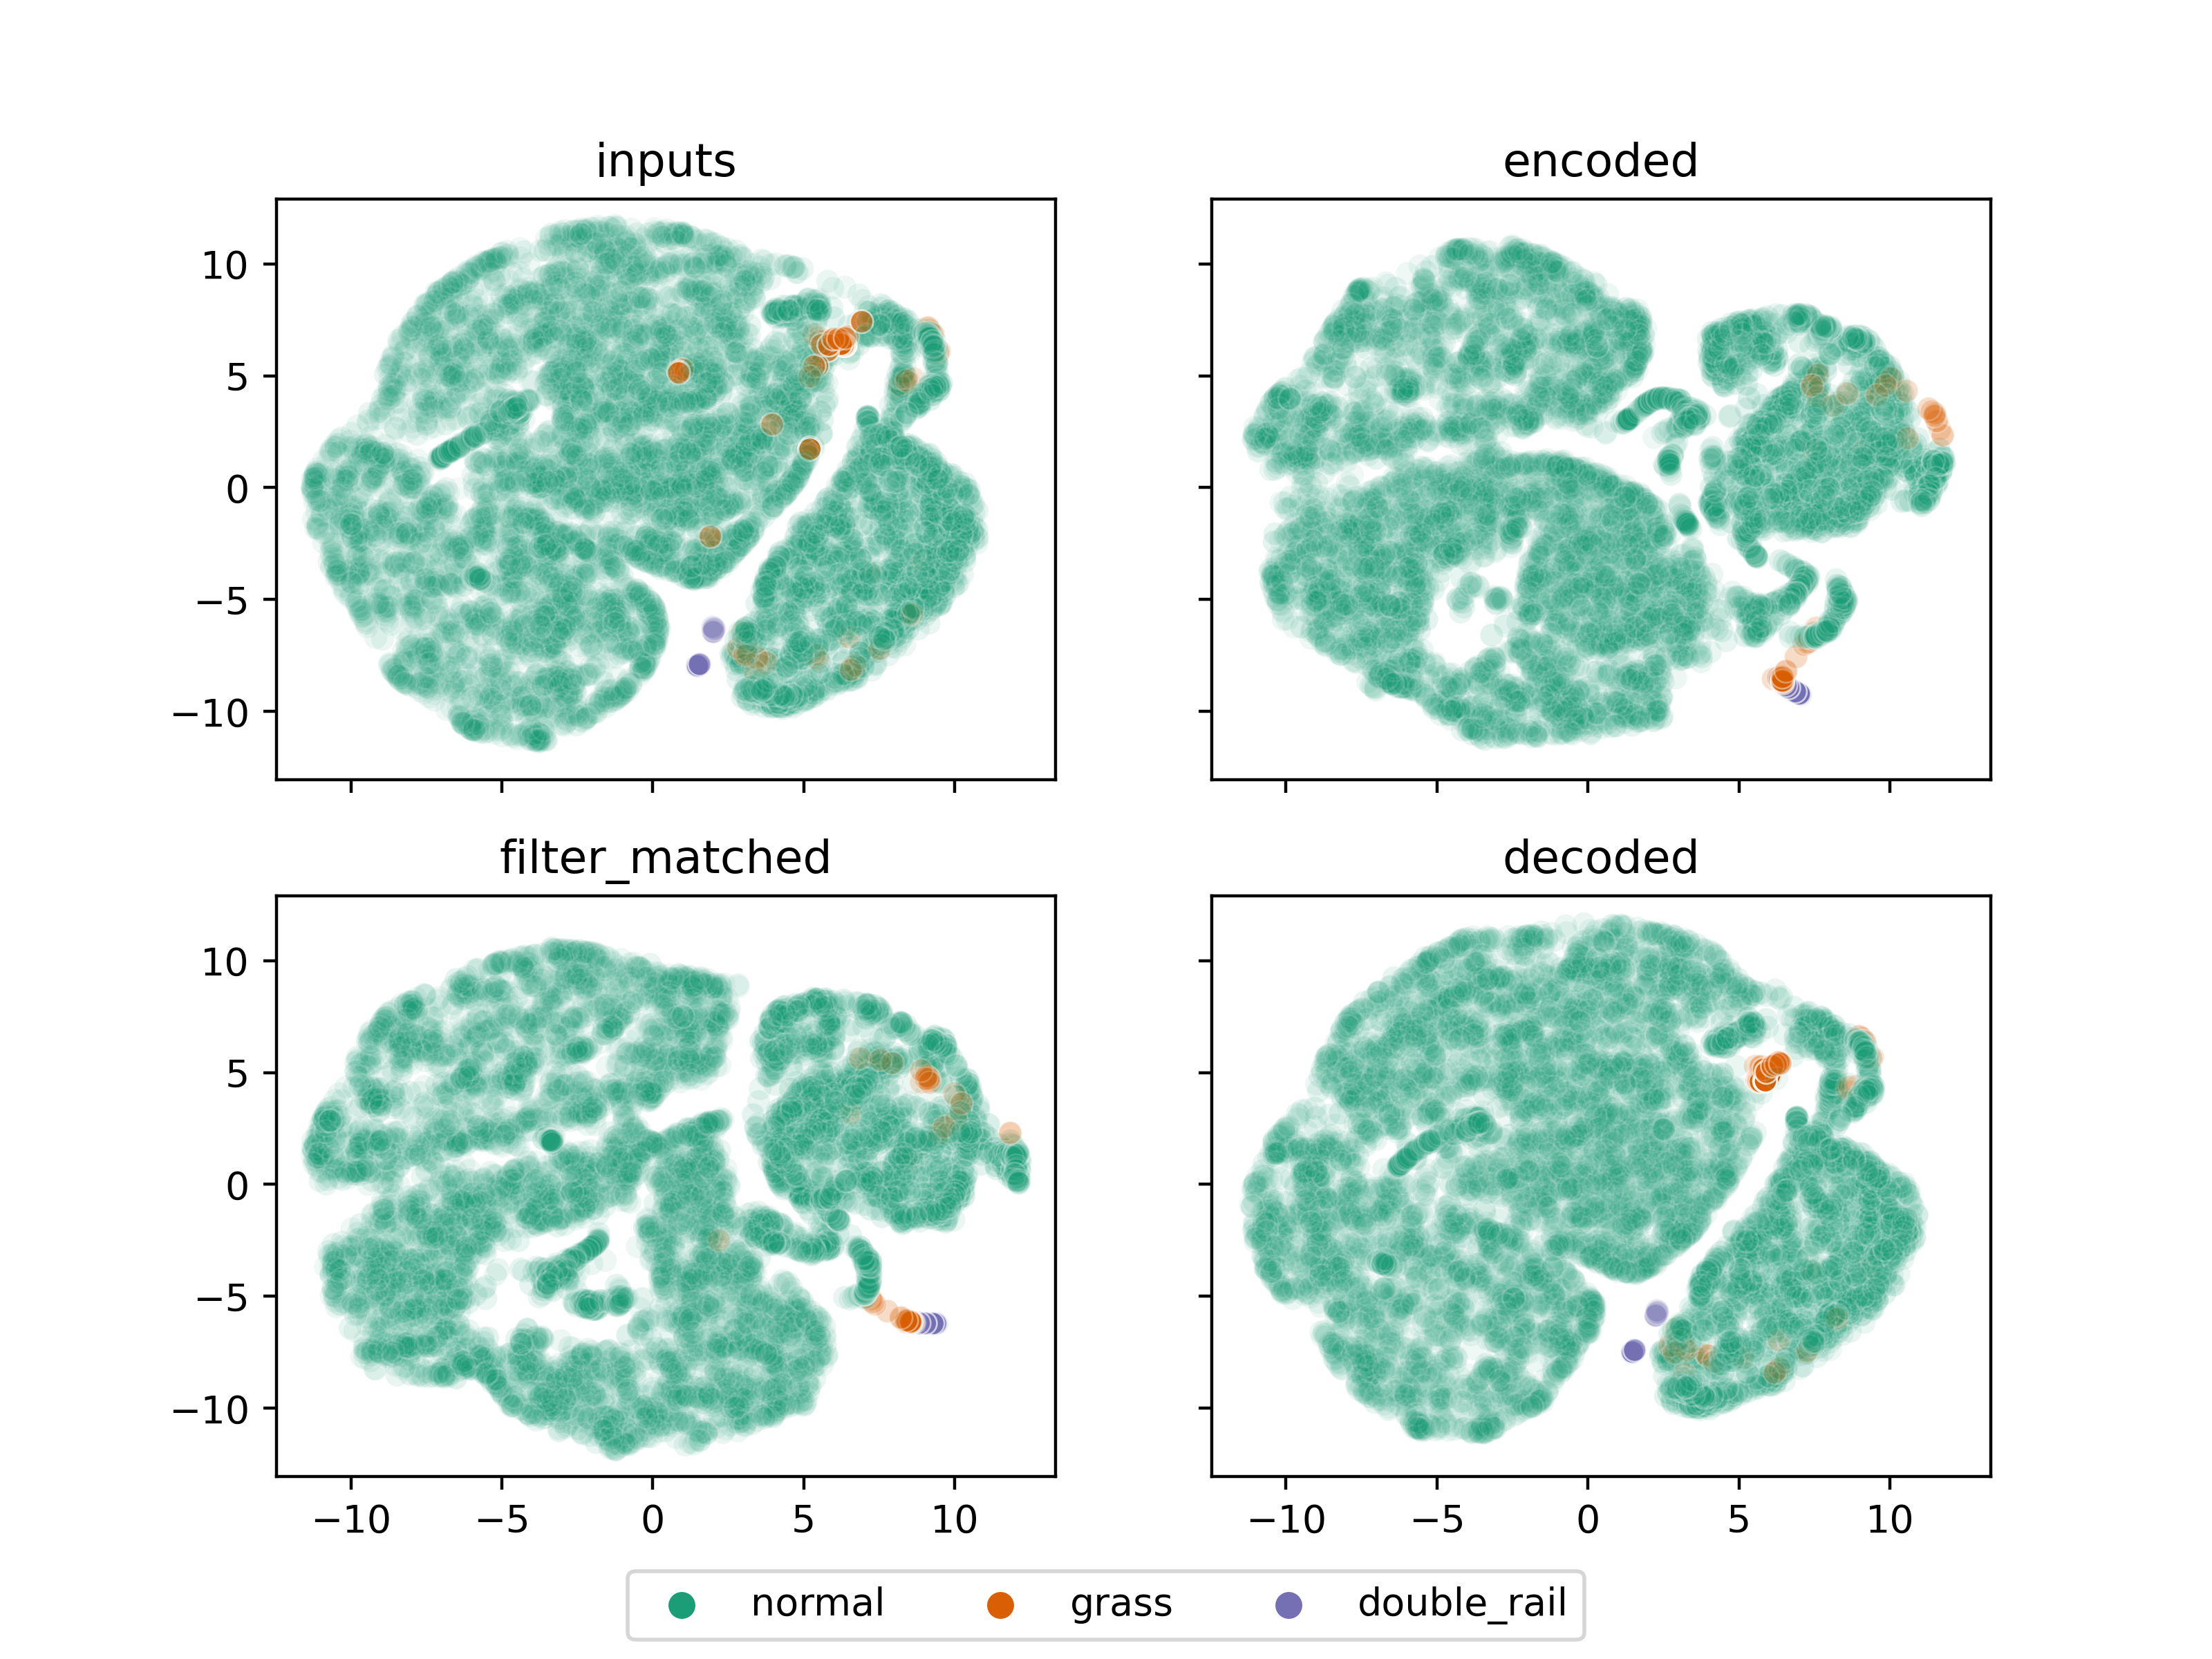
\includegraphics[width=\textwidth,trim={0 0 0 1cm},clip]{./results/efficientnetv2l_vgg19/20230525_194238_feature_vectors_1.png}
    \caption{PCA / t-SNE visualization of the EfficientNetV2L Encoder}
    \label{fig:efficientnetv2l_pca}
\end{figure}

The loss values of the full dataset is shown on Figure \ref{fig:efficientnetv2l_loss}.
Once again the same characteristics can be seen as for the other models.
The loss metric alone is not necessarily indicates the performance of these anomaly detectors.
Most of the outliers can be found by comparing the loss values with a given threshold,
however some of those remain embedded and can not be retained with this method.

\begin{figure}[!ht]
    \centering
    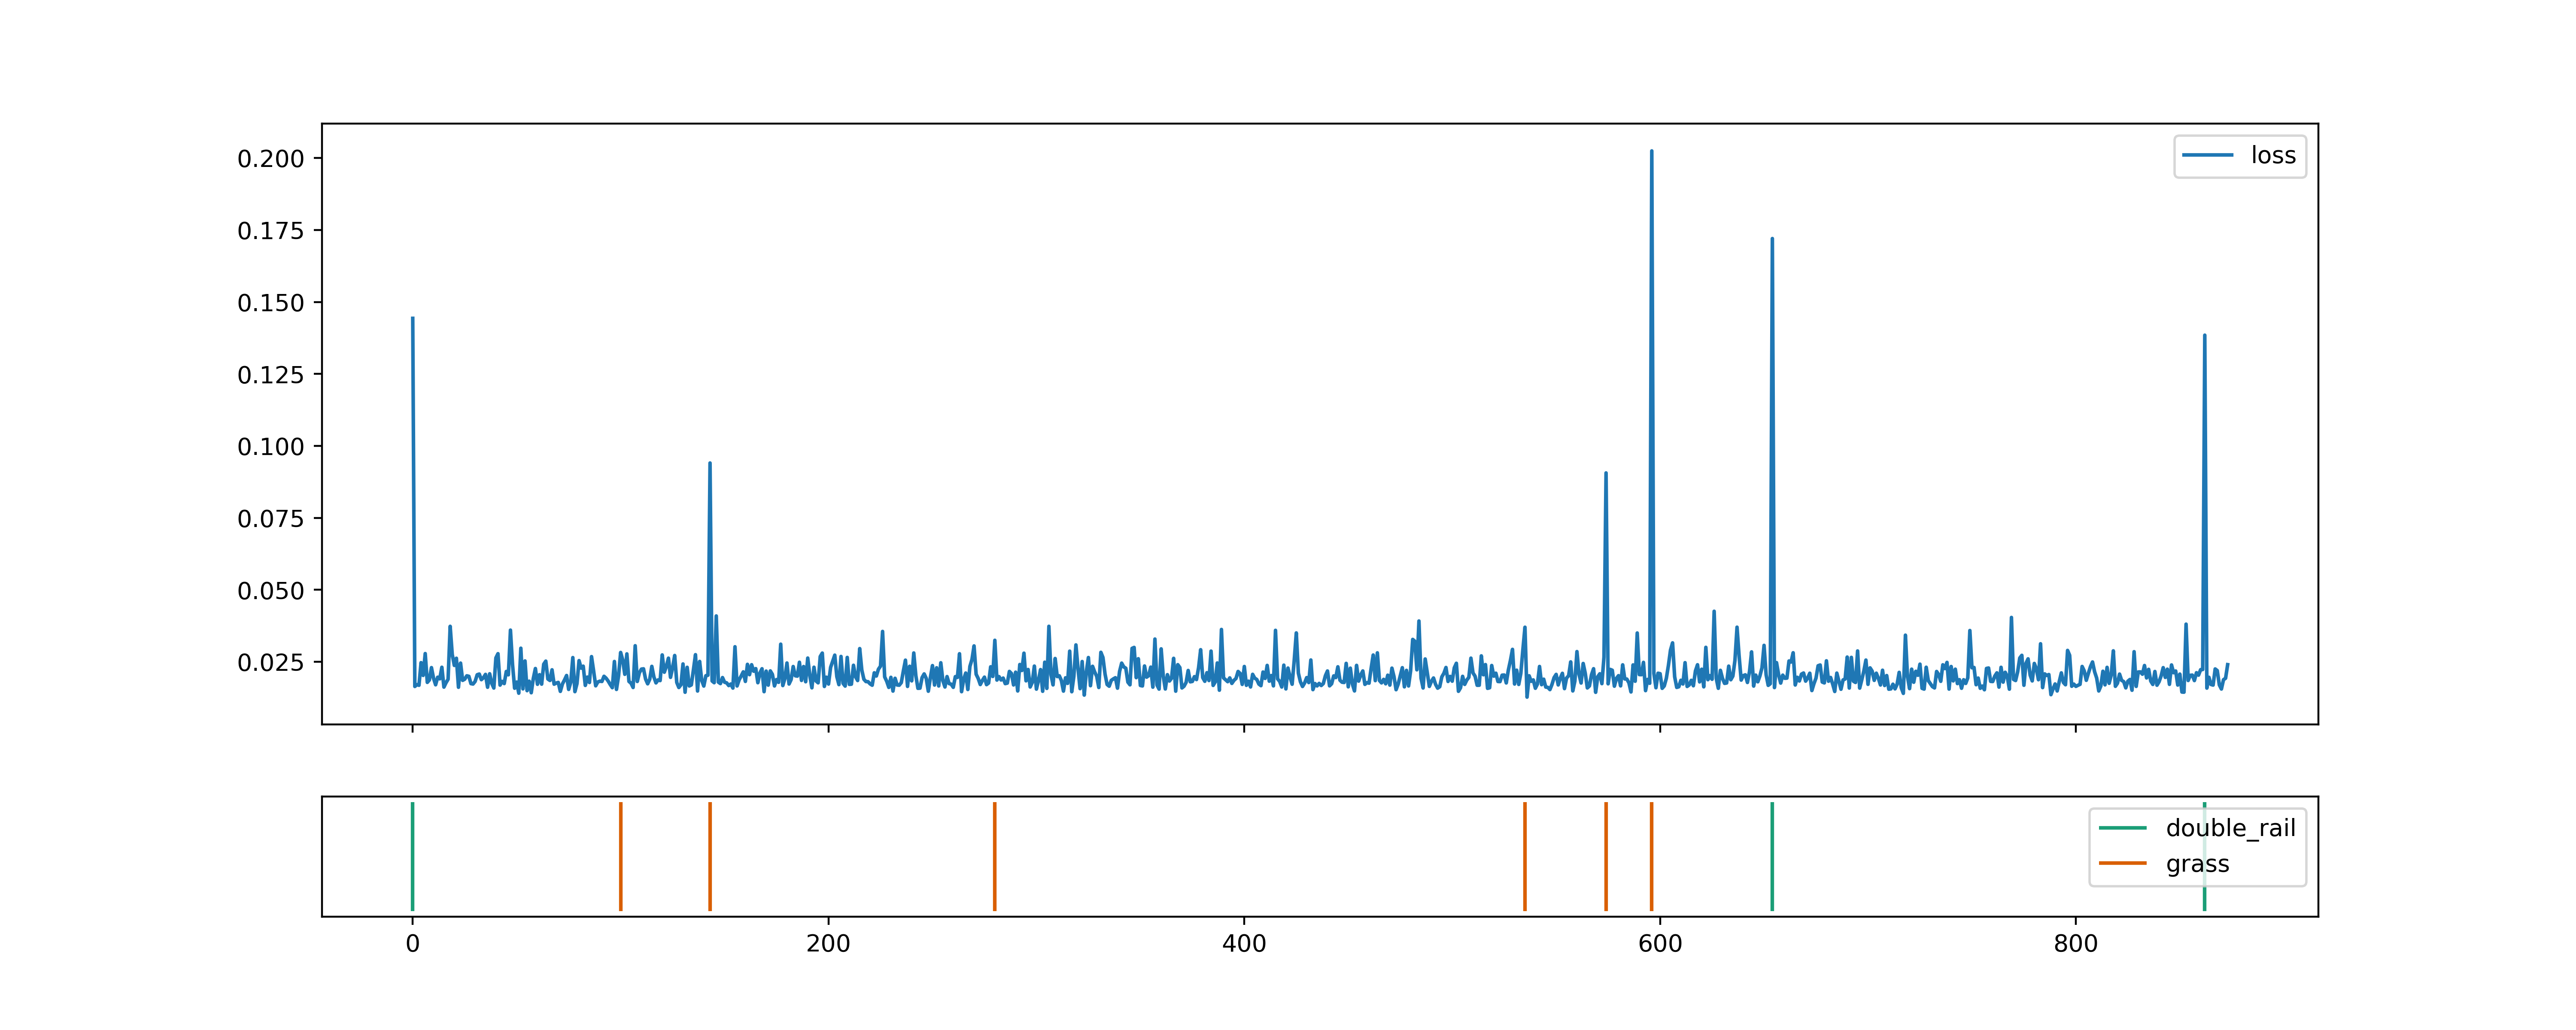
\includegraphics[width=\textwidth,trim={0 1cm 0 1cm},clip]{./results/efficientnetv2l_vgg19/20230525_194238_feature_vectors_loss.png}
    \caption{Loss values of the dataset with EfficientNetV2L encoding}
    \label{fig:efficientnetv2l_loss}
\end{figure}

The classification metrics as shown with the confusion matrices on Figure \ref{fig:efficientnetv2l_cm}
present a similar performance of the loss-based approach,
a little bit more than \small \sfrac{2}{3} of the outliers found.
The Isolation Forest delivers one of the best true positive indications,
but on the cost of worst false negative rate.

\begin{figure}[!ht]
    \centering
    \begin{subfigure}{0.4\textwidth}
        \centering
        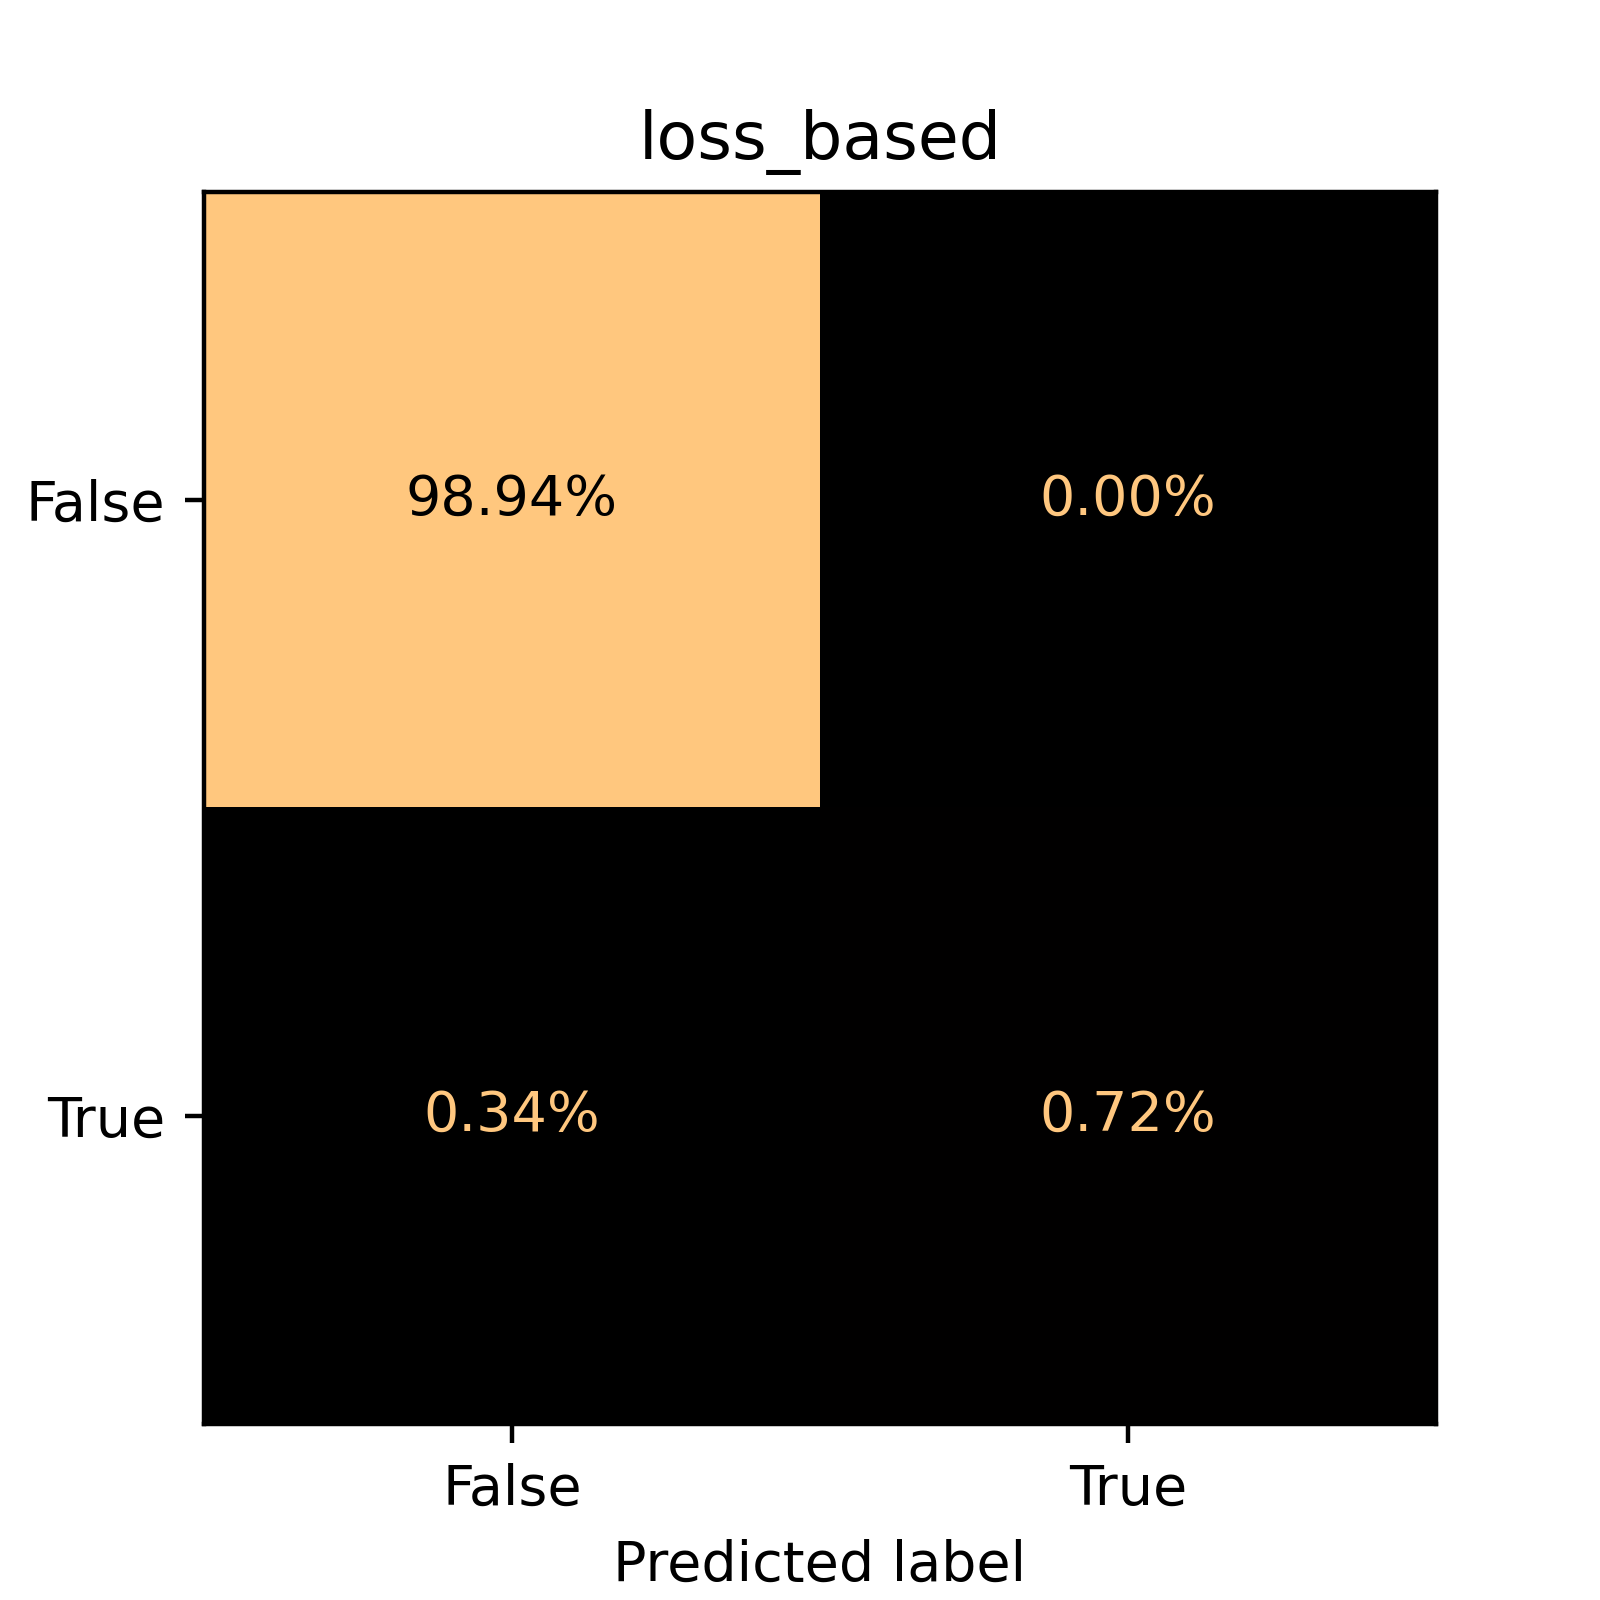
\includegraphics[width=\textwidth]{./results/efficientnetv2l_vgg19/20230525_194238_loss_based_cm.png}
    \end{subfigure}
    \begin{subfigure}{0.4\textwidth}
        \centering
        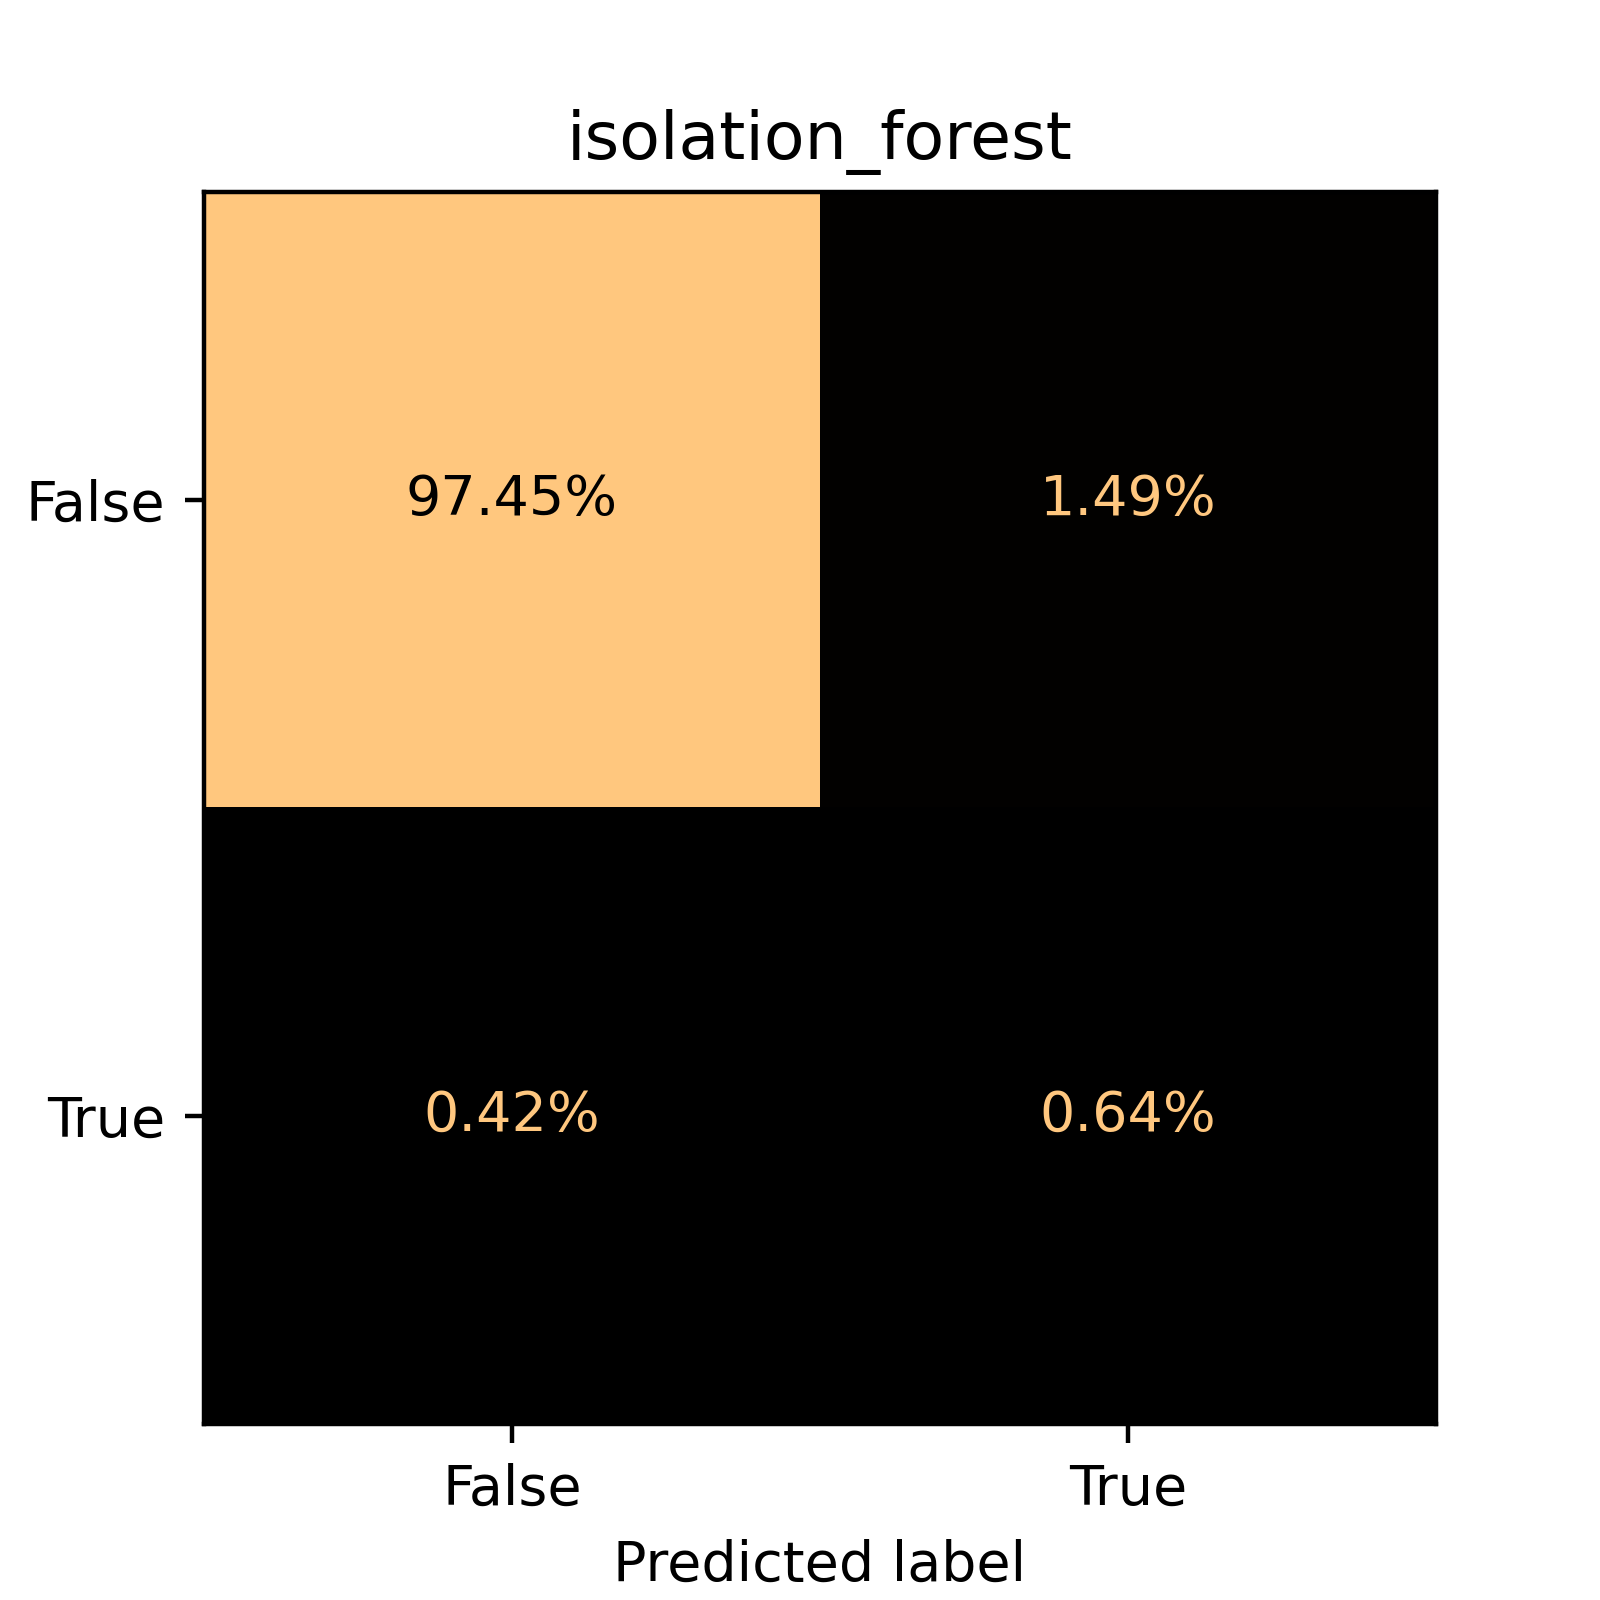
\includegraphics[width=\textwidth]{./results/efficientnetv2l_vgg19/20230525_194238_isolation_forest_cm.png}
    \end{subfigure}
    \caption{Confusion Matrices of the EfficientNetV2L Encoder}
    \label{fig:efficientnetv2l_cm}
\end{figure}